\begin{frame}[t]{Lessons}

  \pause

  \begin{center}
    \large{Scalability != Performance}\\
    \vspace{0.1cm}
    \textit{"Can it scale well?"} - not the right question!
  \end{center}
  
  \vspace{0.5cm}
  \pause
  
  Before you build a big data system,
  \vspace{0.1cm}
  \begin{itemize}
    \item Beware of misleading marketing. "One tool for all screws"
    \item Self-investigation is necessary.
    \item Use appropriate algorithms.
    \item Choose to solve the problem locally,\\ don't distribute unless absolutely necessary.
  \end{itemize}

\end{frame}

\begin{frame}[t]{Interesting stuff}

  \vspace{0.25cm}

  Further reading:
  \vspace{0.25cm}
  \begin{itemize}
    \item Boruvka’s algorithm
    \item Galois and Ligra systems
    \item Naiad - timely dataflow
  \end{itemize}

  \vspace{0.5cm}

  People/Things to follow:\\
  \vspace{0.25cm}
  \textbf{Frank McSherry} - https://github.com/frankmcsherry/\\
  \vspace{0.30cm}
  \textbf{Kyle Kingsbury} - https://aphyr.com/\\
  \vspace{0.25cm}
  \textbf{Jepsen} - https://github.com/jepsen-io/jepsen 

\end{frame}

\begin{frame}[t]{Interesting stuff}

  \vspace{0.25cm}

  \begin{center}
    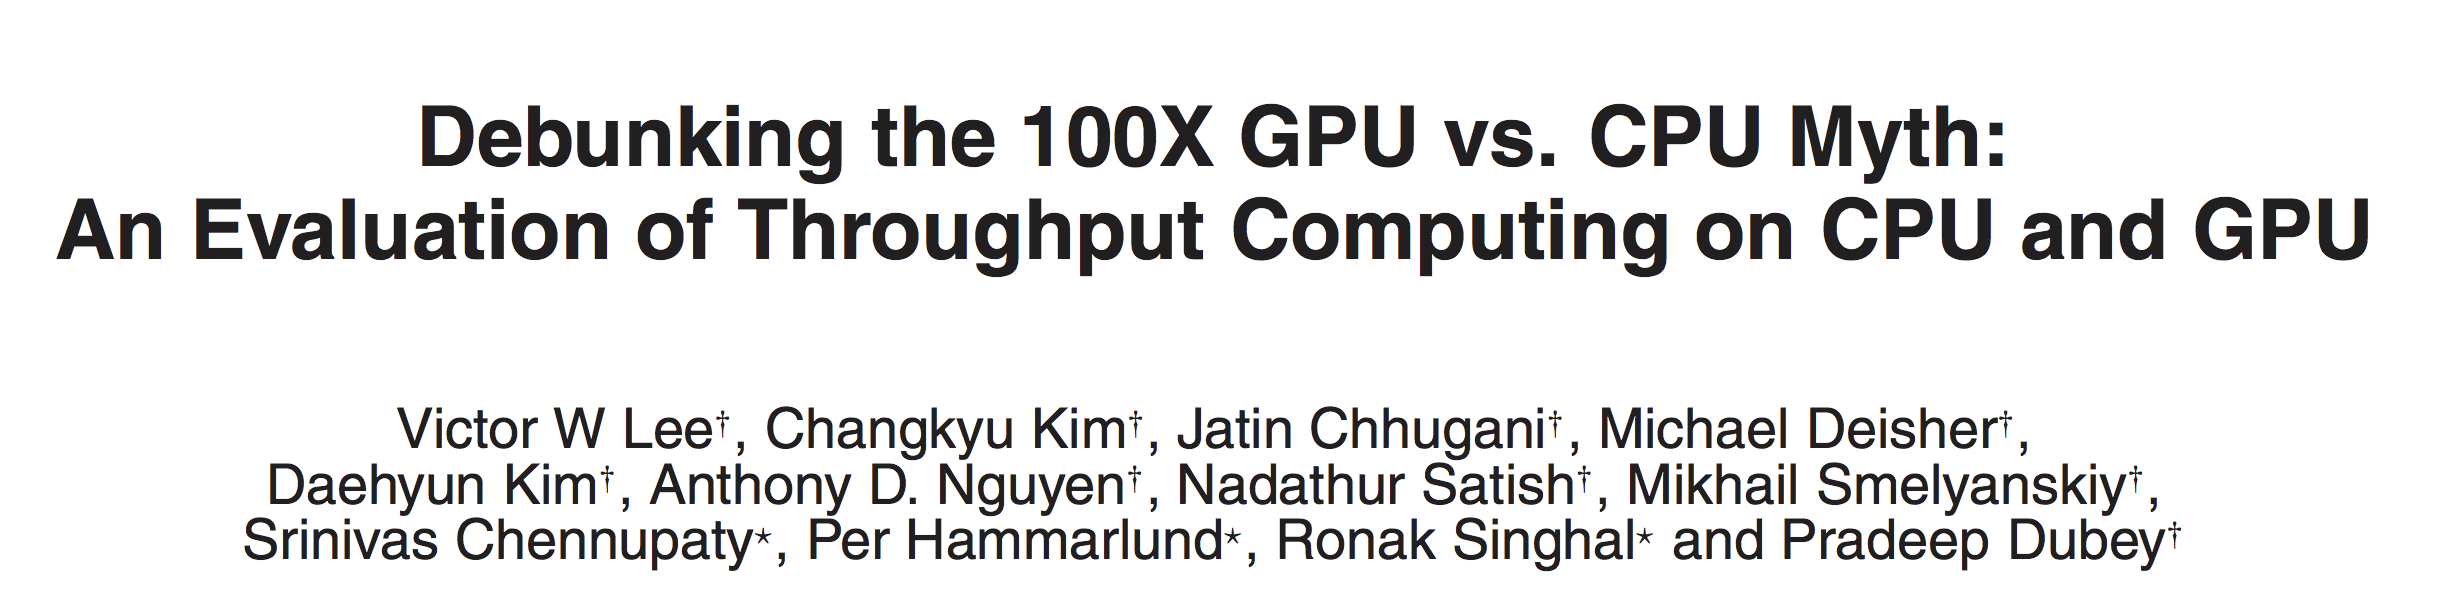
\includegraphics[width=0.80\textwidth]{debunking}
  \end{center}

\end{frame}


